% Week 1: Foundations and Statistical Language Modeling
% Using the Master Optimal Readability Template

% Master Template for NLP Course
% Optimal Readability Layout Standard
% All presentations should include this template

\documentclass[8pt,aspectratio=169]{beamer}
\usetheme{Madrid}
\setbeamertemplate{navigation symbols}{}

% ====================================
% OPTIMAL READABILITY COLOR PALETTE
% ====================================
\definecolor{PureBlack}{HTML}{000000}      % Main text (21:1 contrast)
\definecolor{DeepBlue}{HTML}{003D7A}       % Primary accent (12.6:1 contrast)
\definecolor{DarkGray}{HTML}{4A4A4A}       % Secondary text (9.7:1 contrast)
\definecolor{LightGray}{HTML}{E5E5E5}      % Borders and grids
\definecolor{ChartBlue}{HTML}{0066CC}      % Chart primary
\definecolor{ChartOrange}{HTML}{FF8800}    % Chart secondary
\definecolor{ChartTeal}{HTML}{00A0A0}      % Chart tertiary
\definecolor{ChartPurple}{HTML}{8B4789}    % Chart quaternary
\definecolor{DarkGreen}{HTML}{228B22}      % Success/positive
\definecolor{DarkRed}{HTML}{CC0000}        % Warning/negative

% ====================================
% BEAMER COLOR CONFIGURATION
% ====================================
\setbeamercolor{structure}{fg=PureBlack}
\setbeamercolor{frametitle}{fg=PureBlack,bg=white}
\setbeamercolor{title}{fg=PureBlack,bg=white}
\setbeamercolor{subtitle}{fg=DarkGray}
\setbeamercolor{author}{fg=DarkGray}
\setbeamercolor{date}{fg=DarkGray}
\setbeamercolor{institute}{fg=DarkGray}

% Blocks - no backgrounds
\setbeamercolor{block title}{fg=PureBlack,bg=white}
\setbeamercolor{block body}{fg=PureBlack,bg=white}
\setbeamercolor{block title example}{fg=DarkGreen,bg=white}
\setbeamercolor{block body example}{fg=PureBlack,bg=white}
\setbeamercolor{block title alerted}{fg=DarkRed,bg=white}
\setbeamercolor{block body alerted}{fg=PureBlack,bg=white}

% Lists
\setbeamercolor{item}{fg=DeepBlue}
\setbeamercolor{subitem}{fg=ChartBlue}
\setbeamercolor{enumerate item}{fg=DeepBlue}
\setbeamercolor{enumerate subitem}{fg=ChartBlue}

% Text
\setbeamercolor{normal text}{fg=PureBlack,bg=white}
\setbeamercolor{alerted text}{fg=DarkRed}
\setbeamercolor{example text}{fg=DarkGreen}

% Footer
\setbeamercolor{footline}{fg=DarkGray,bg=white}
\setbeamercolor{page number in head/foot}{fg=DarkGray}

% ====================================
% FONT CONFIGURATION
% ====================================
\setbeamerfont{normal text}{size=\normalsize}
\setbeamerfont{frametitle}{size=\Large,series=\bfseries}
\setbeamerfont{title}{size=\huge,series=\bfseries}
\setbeamerfont{subtitle}{size=\large}
\setbeamerfont{author}{size=\normalsize}
\setbeamerfont{date}{size=\small}
\setbeamerfont{institute}{size=\small}

% ====================================
% REQUIRED PACKAGES
% ====================================
\usepackage{tikz}
\usepackage{amsmath}
\usepackage{amssymb}
\usepackage{booktabs}
\usepackage{graphicx}
\usepackage{array}
\usepackage{listings}
\usepackage{algorithm2e}
\usepackage{xcolor}
\usepackage{tabularx}
\usepackage{multirow}
\usepackage{subcaption}

% ====================================
% CUSTOM COMMANDS
% ====================================
% Text highlighting commands
\newcommand{\highlight}[1]{\textcolor{DeepBlue}{\textbf{#1}}}
\newcommand{\secondary}[1]{\textcolor{DarkGray}{#1}}
\newcommand{\success}[1]{\textcolor{DarkGreen}{#1}}
\newcommand{\warning}[1]{\textcolor{DarkRed}{#1}}
\newcommand{\data}[1]{\textcolor{ChartBlue}{#1}}
\newcommand{\dataalt}[1]{\textcolor{ChartOrange}{#1}}

% Mathematical notation
\newcommand{\given}{\mid}
\newcommand{\prob}[1]{P(#1)}
\newcommand{\argmax}{\operatorname*{argmax}}
\newcommand{\argmin}{\operatorname*{argmin}}
\newcommand{\softmax}{\operatorname{softmax}}

% Box commands for emphasis
\newcommand{\keypoint}[1]{%
  \begin{center}
  \fbox{\parbox{0.9\textwidth}{\centering\textbf{#1}}}
  \end{center}
}

\newcommand{\formula}[1]{%
  \begin{center}
  \colorbox{LightGray}{\parbox{0.8\textwidth}{\centering$\displaystyle #1$}}
  \end{center}
}

% ====================================
% LISTINGS CONFIGURATION
% ====================================
\lstset{
  basicstyle=\ttfamily\small,
  keywordstyle=\color{DeepBlue}\bfseries,
  commentstyle=\color{DarkGray}\itshape,
  stringstyle=\color{ChartOrange},
  numbers=left,
  numberstyle=\tiny\color{DarkGray},
  stepnumber=1,
  numbersep=5pt,
  backgroundcolor=\color{white},
  showspaces=false,
  showstringspaces=false,
  showtabs=false,
  frame=single,
  frameround=tttt,
  rulecolor=\color{LightGray},
  tabsize=2,
  captionpos=b,
  breaklines=true,
  breakatwhitespace=true,
  language=Python,
  escapeinside={(*@}{@*)},
  morekeywords={self, yield, assert, with, as}
}

% ====================================
% STANDARD SLIDE LAYOUTS
% ====================================

% Two-column layout with title
\newcommand{\twocolslide}[3]{%
  \begin{frame}{#1}
  \begin{columns}[T]
  \column{0.48\textwidth}
  #2
  \column{0.48\textwidth}
  #3
  \end{columns}
  \end{frame}
}

% Three-column layout
\newcommand{\threecolslide}[4]{%
  \begin{frame}{#1}
  \begin{columns}[T]
  \column{0.32\textwidth}
  #2
  \column{0.32\textwidth}
  #3
  \column{0.32\textwidth}
  #4
  \end{columns}
  \end{frame}
}

% Chart slide with caption
\newcommand{\chartslide}[3]{%
  \begin{frame}{#1}
  \begin{center}
  \includegraphics[width=#2\textwidth]{#3}
  \end{center}
  \end{frame}
}

% Full chart slide - optimized to 0.85 for proper margins
\newcommand{\fullchartslide}[2]{%
  \begin{frame}{#1}
  \begin{center}
  \includegraphics[width=0.85\textwidth]{#2}
  \end{center}
  \end{frame}
}

% Code slide
\newcommand{\codeslide}[3]{%
  \begin{frame}[fragile]{#1}
  \begin{lstlisting}[language=#2]
#3
  \end{lstlisting}
  \end{frame}
}

% Concept slide with figure
\newcommand{\conceptslide}[3]{%
  \begin{frame}{#1}
  \begin{columns}[T]
  \column{0.6\textwidth}
  #2
  \column{0.35\textwidth}
  \begin{center}
  \includegraphics[width=0.95\textwidth]{#3}
  \end{center}
  \end{columns}
  \end{frame}
}

% Table slide
\newcommand{\tableslide}[2]{%
  \begin{frame}{#1}
  \begin{center}
  \Large
  \renewcommand{\arraystretch}{1.5}
  #2
  \end{center}
  \end{frame}
}

% Summary slide
\newcommand{\summaryslide}[2]{%
  \begin{frame}{#1}
  \begin{center}
  \Large
  #2
  \end{center}
  \vfill
  \begin{center}
  \keypoint{Key Takeaway}
  \end{center}
  \end{frame}
}

% ====================================
% REMOVE DECORATIONS
% ====================================
\setbeamertemplate{blocks}[default]
\setbeamertemplate{title page}[default][colsep=-4bp,rounded=false]
\setbeamertemplate{itemize items}[circle]
\setbeamertemplate{enumerate items}[default]
\setbeamertemplate{section in toc}[sections numbered]
\setbeamertemplate{subsection in toc}[subsections numbered]

% ====================================
% PAGE NUMBERING
% ====================================
\setbeamertemplate{footline}{
  \leavevmode%
  \hbox{%
  \begin{beamercolorbox}[wd=.333333\paperwidth,ht=2.25ex,dp=1ex,center]{author in head/foot}%
    \usebeamerfont{author in head/foot}\secondary{\insertshortauthor}
  \end{beamercolorbox}%
  \begin{beamercolorbox}[wd=.333333\paperwidth,ht=2.25ex,dp=1ex,center]{title in head/foot}%
    \usebeamerfont{title in head/foot}\secondary{\insertshorttitle}
  \end{beamercolorbox}%
  \begin{beamercolorbox}[wd=.333333\paperwidth,ht=2.25ex,dp=1ex,right]{date in head/foot}%
    \usebeamerfont{date in head/foot}\secondary{\insertshortdate{}\hspace*{2em}
    \insertframenumber{} / \inserttotalframenumber\hspace*{2ex}}
  \end{beamercolorbox}}%
  \vskip0pt%
}

% ====================================
% TABLE OF CONTENTS STYLE
% ====================================
\setbeamertemplate{section in toc}{%
  \leavevmode\leftskip=1.5em%
  \llap{%
    \usebeamerfont{section in toc}%
    \usebeamercolor[fg]{section in toc}%
    \inserttocsectionnumber.%
  }%
  \usebeamerfont{section in toc}%
  \usebeamercolor[fg]{section in toc}%
  \inserttocsection\par%
}

\setbeamertemplate{subsection in toc}{%
  \leavevmode\leftskip=3em%
  \llap{%
    \usebeamerfont{subsection in toc}%
    \usebeamercolor[fg]{subsection in toc}%
    \inserttocsectionnumber.\inserttocsubsectionnumber%
  }%
  \usebeamerfont{subsection in toc}%
  \usebeamercolor[fg]{subsection in toc}%
  \inserttocsubsection\par%
}

% ====================================
% END OF MASTER TEMPLATE
% ====================================

\title{Foundations of NLP}
\subtitle{\secondary{Week 1 - Statistical Language Modeling}}
\author{NLP Course 2025}
\date{\today}

\begin{document}

% Title slide
\begin{frame}
\titlepage
\vfill
\begin{center}
\secondary{\footnotesize Using Optimal Readability Template}
\end{center}
\end{frame}

% Overview using three columns
\threecolslide{Course Overview}{
  \textbf{Foundations}
  \begin{itemize}
  \item Language basics
  \item Probability theory
  \item N-gram models
  \item Evaluation metrics
  \end{itemize}
}{
  \textbf{Neural Methods}
  \begin{itemize}
  \item Word embeddings
  \item RNNs and LSTMs
  \item Seq2Seq models
  \item Attention mechanism
  \end{itemize}
}{
  \textbf{Modern NLP}
  \begin{itemize}
  \item Transformers
  \item Pre-training
  \item Fine-tuning
  \item Applications
  \end{itemize}
}

% Concept slide with key points
\begin{frame}{What is Language Modeling?}
\begin{columns}[T]
\column{0.6\textwidth}
\textbf{Core Objective}
\begin{itemize}
\item Assign \highlight{probabilities} to sequences of words
\item Predict the \data{next word} given context
\item Model the \secondary{structure} of language
\end{itemize}

\vspace{5mm}
\textbf{Applications}
\begin{itemize}
\item \success{Machine Translation}
\item \success{Speech Recognition}
\item \success{Text Generation}
\item \success{Spell Correction}
\end{itemize}

\column{0.35\textwidth}
\keypoint{Language models capture the statistical patterns in text}

\vspace{5mm}
\formula{P(w_1, w_2, ..., w_n)}
\end{columns}
\end{frame}

% Two-column mathematical content
\twocolslide{Probability Fundamentals}{
  \textbf{Chain Rule}
  \begin{align*}
  P(w_1^n) &= P(w_1) \times P(w_2|w_1) \\
  &\times P(w_3|w_1^2) ... P(w_n|w_1^{n-1})
  \end{align*}

  \textbf{Markov Assumption}
  $$P(w_i|w_1^{i-1}) \approx P(w_i|w_{i-k+1}^{i-1})$$
}{
  \textbf{N-gram Models}
  \begin{itemize}
  \item \highlight{Unigram}: $P(w_i)$
  \item \highlight{Bigram}: $P(w_i|w_{i-1})$
  \item \highlight{Trigram}: $P(w_i|w_{i-2}, w_{i-1})$
  \end{itemize}

  \vspace{5mm}
  \secondary{Trade-off: Context vs Sparsity}
}

% Table slide
\tableslide{N-gram Model Comparison}{
  \begin{tabular}{l|ccc|c}
  \toprule
  \textbf{Model} & \textbf{Context} & \textbf{Parameters} & \textbf{Sparsity} & \textbf{Perplexity} \\
  \midrule
  Unigram & 0 words & $V$ & \success{Low} & \warning{250} \\
  Bigram & 1 word & $V^2$ & Medium & \data{120} \\
  Trigram & 2 words & $V^3$ & \warning{High} & \data{85} \\
  4-gram & 3 words & $V^4$ & \warning{Very High} & \highlight{72} \\
  \bottomrule
  \multicolumn{5}{l}{\secondary{\footnotesize $V$ = Vocabulary size (typically 10,000-50,000)}}
  \end{tabular}
}

% Code example
\begin{frame}[fragile]{Implementation Example}
\begin{columns}[T]
\column{0.55\textwidth}
\begin{lstlisting}[language=Python]
class BigramModel:
    def __init__(self):
        self.counts = defaultdict(
            lambda: defaultdict(int)
        )
        self.vocab = set()

    def train(self, text):
        words = text.split()
        for i in range(len(words)-1):
            w1, w2 = words[i], words[i+1]
            self.counts[w1][w2] += 1
            self.vocab.update([w1, w2])

    def probability(self, w1, w2):
        if w1 not in self.counts:
            return 0.0
        total = sum(self.counts[w1].values())
        return self.counts[w1][w2] / total
\end{lstlisting}

\column{0.42\textwidth}
\textbf{Key Components}
\begin{itemize}
\item \highlight{counts}: Store bigram frequencies
\item \highlight{vocab}: Track unique words
\item \data{train()}: Build frequency table
\item \data{probability()}: Calculate $P(w_2|w_1)$
\end{itemize}

\vspace{5mm}
\textbf{Complexity}
\begin{itemize}
\item Time: \success{O(n)} for training
\item Space: \warning{O($V^2$)} worst case
\item Query: \success{O(1)} lookup
\end{itemize}
\end{columns}
\end{frame}

% Evaluation metrics
\begin{frame}{Evaluation Metrics}
\begin{columns}[T]
\column{0.48\textwidth}
\textbf{Perplexity}
\formula{PP(W) = P(w_1 w_2 ... w_N)^{-\frac{1}{N}}}

\begin{itemize}
\item \highlight{Lower is better}
\item Geometric mean of inverse probability
\item Typical ranges: 50-500
\end{itemize}

\vspace{5mm}
\textbf{Interpretation}
\begin{itemize}
\item PP = 100: \secondary{On average, choosing from 100 equally likely words}
\item PP = 10: \success{Very good model}
\item PP = 1000: \warning{Poor model}
\end{itemize}

\column{0.48\textwidth}
\textbf{Cross-Entropy}
\formula{H(P, Q) = -\sum_x P(x) \log Q(x)}

\begin{itemize}
\item Measures \data{information loss}
\item Related: $PP = 2^H$
\item Used in neural models
\end{itemize}

\vspace{5mm}
\textbf{Other Metrics}
\begin{itemize}
\item \data{BLEU}: Machine translation
\item \data{ROUGE}: Summarization
\item \data{Word Error Rate}: Speech
\end{itemize}
\end{columns}
\end{frame}

% Smoothing techniques
\begin{frame}{Smoothing Techniques}
\begin{center}
\Large
\textbf{The Zero Probability Problem}
\end{center}

\vspace{5mm}

\begin{columns}[T]
\column{0.32\textwidth}
\textbf{Add-One (Laplace)}
$$P(w_i|w_{i-1}) = \frac{c(w_{i-1}, w_i) + 1}{c(w_{i-1}) + V}$$

\begin{itemize}
\item Simple to implement
\item \warning{Over-smooths}
\item Poor performance
\end{itemize}

\column{0.32\textwidth}
\textbf{Good-Turing}
$$c^* = (c+1) \frac{N_{c+1}}{N_c}$$

\begin{itemize}
\item Better estimates
\item \data{Complex theory}
\item Works well
\end{itemize}

\column{0.32\textwidth}
\textbf{Kneser-Ney}
$$P_{KN}(w_i|w_{i-1}) = \frac{\max(c - d, 0)}{c(w_{i-1})} + \lambda P_{cont}(w_i)$$

\begin{itemize}
\item \success{State-of-the-art}
\item Interpolation-based
\item Best results
\end{itemize}
\end{columns}

\vfill
\keypoint{Smoothing redistributes probability mass to unseen events}
\end{frame}

% Historical context
\begin{frame}{Historical Perspective}
\begin{center}
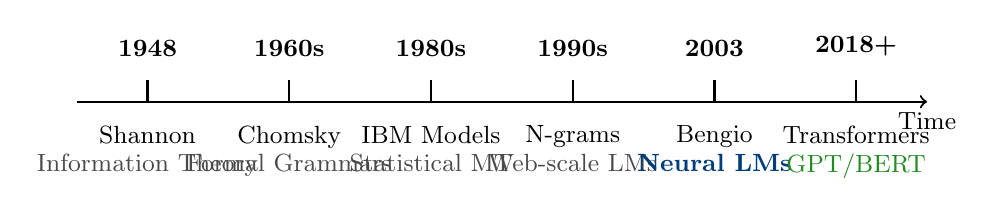
\begin{tikzpicture}[scale=0.9, every node/.style={font=\small}]
% Timeline
\draw[thick, ->, color=black] (0,0) -- (12,0) node[anchor=north] {Time};

% Events
\node[above] at (1,0.5) {\textbf{1948}};
\node[below] at (1,-0.2) {Shannon};
\node[below] at (1,-0.6) {\secondary{Information Theory}};

\node[above] at (3,0.5) {\textbf{1960s}};
\node[below] at (3,-0.2) {Chomsky};
\node[below] at (3,-0.6) {\secondary{Formal Grammars}};

\node[above] at (5,0.5) {\textbf{1980s}};
\node[below] at (5,-0.2) {IBM Models};
\node[below] at (5,-0.6) {\secondary{Statistical MT}};

\node[above] at (7,0.5) {\textbf{1990s}};
\node[below] at (7,-0.2) {N-grams};
\node[below] at (7,-0.6) {\secondary{Web-scale LMs}};

\node[above] at (9,0.5) {\textbf{2003}};
\node[below] at (9,-0.2) {Bengio};
\node[below] at (9,-0.6) {\highlight{Neural LMs}};

\node[above] at (11,0.5) {\textbf{2018+}};
\node[below] at (11,-0.2) {Transformers};
\node[below] at (11,-0.6) {\success{GPT/BERT}};

% Markers
\foreach \x in {1,3,5,7,9,11} {
  \draw[thick] (\x,0) -- (\x,0.3);
}
\end{tikzpicture}
\end{center}

\vspace{10mm}
\begin{center}
\Large
\highlight{From Rules} $\rightarrow$ \data{Statistics} $\rightarrow$ \success{Deep Learning}
\end{center}
\end{frame}

% Summary
\summaryslide{Week 1 Summary}{
  \begin{itemize}
  \item Language modeling assigns \highlight{probabilities} to text
  \item N-gram models use \data{Markov assumption} for tractability
  \item \warning{Sparsity} is the main challenge
  \item \success{Smoothing} techniques handle unseen events
  \item Evaluation via \data{perplexity} and cross-entropy
  \end{itemize}

  \vspace{10mm}
  \textbf{Next Week:} Neural Language Models \& Word Embeddings
}

\end{document}